\documentclass{standalone}
%
\usepackage{tikz}
\usetikzlibrary{backgrounds,arrows.meta,shapes.callouts}
\usepackage{xcolor}
%
\definecolor{space}{HTML}{1F2C4E}
\definecolor{earth}{HTML}{0089FA}
\definecolor{dida}{HTML}{FFDE00}
\definecolor{title}{HTML}{FBA706}
\definecolor{galaxy}{HTML}{4278A4}
\definecolor{paper01}{HTML}{BE8A3F}
\definecolor{paper02}{HTML}{E5D09B}
%
\usepackage{fontspec}
\setmainfont{Open Dyslexic}
%
\title{Vite da ricordare}
\begin{document}
	\begin{tikzpicture}[background rectangle/.style={fill=white},show background rectangle,>={[inset=0,angle'=27]Stealth}]
		% title
		\draw [black,ultra thick,fill=title] (0,12.8) rectangle (30,16.8);
		\node at (15,14.8) {\textcolor{black}{\fontsize{75}{76}\selectfont Vite da ricordare}};
		% stripe
		\begin{scope}[shift={(0,12)}]
			\draw [fill=earth!50!white, thick] (14.5,0) rectangle (26.5,-198.5);
			\foreach \i in {0,1,...,11}
			{
				\draw [fill=white, thick] (14.75+\i,-0.5) rectangle (15.25+\i,-1);
			}
			%
			\foreach \j in {0,1,...,11}
			{
				\draw [fill=white, thick] (14.75+\j,-196.5) rectangle (15.25+\j,-197);
			}
		\end{scope}
		%
		% Sophie Brahe
		%
		\begin{scope}[shift={(0,8)}]
			\draw [fill=white, thick] (3,1) rectangle (13,-11);
			\node at (8,-5) {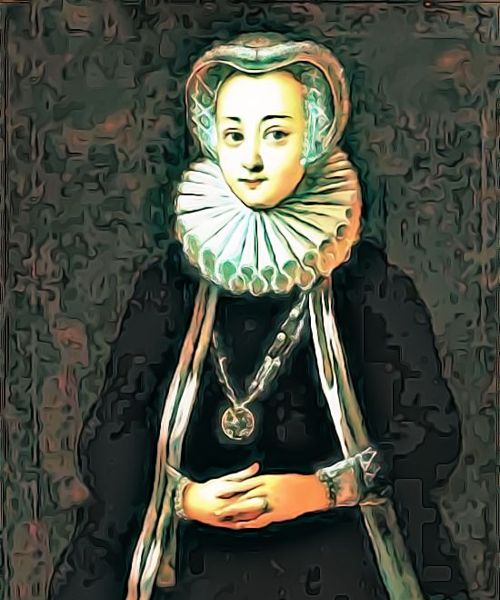
\includegraphics[width=10cm]{img/2026/sophie_brahe.jpg}};
			%
			\draw [fill=galaxy, ultra thick] (3.5,-10.3) rectangle (12.5,-11.4);
			\node at (8,-10.9) {\textcolor{black}{\fontsize{18}{19}\selectfont Sophie Brahe}};
			%
			\draw [fill=title, thick] (14,0.9) rectangle (27,1.8);
			\node (example-textwidth-2) [right, align=left, text width=12cm, color=black, font=\fontsize{18pt}{19pt}\selectfont] at (14.5,1.3) {\textbf{24 agosto 1559-22 settembre 1556}};
			%
			\node (example-textwidth-2) [right, align=left, text width=12cm, color=black, font=\fontsize{18pt}{19pt}\selectfont] at (15,-0.1) {Astronoma};
			%
			\draw [fill=dida, thick] (14,-0.7) rectangle (27,-12.4);
			\node (example-textwidth-2) [right, align=left, text width=11cm, color=black, font=\fontsize{18pt}{19pt}\selectfont] at (15,-6.6) {Sorella del famoso astronomo \textbf{Thyco Brahe}, si interessò di astronomia sin da giovane. Il fratello, pur supportandola nei suoi studi scientifici, non riteneva adatta a lei la carriera di astronoma: pensava, infatti, che non sarebbe stata in grado di redigere gli oroscopi per i ricchi clienti.\\
			Nonostante questo, Sophie studio' sui libri del fratello acquisendo le competenze necessarie per supportarlo nel corso delle sue osservazioni presso l'osservatorio di Uraniborg costruito sull'isola di Ven.};
			%
			\node (example-textwidth-2) [right, align=left, text width=11cm, color=black, font=\fontsize{18pt}{19pt}\selectfont] at (15,-17) {Le capacita' di Sophie vinsero cosi' le resistenze di Thyco, che tra il 1588 e il 1597 le affido' non solo la gestione di Uraniborg, ma anche la stesura degli oroscopi. Nonostante le opposizioni della famiglia (fratello a parte), sposo' in seconde nozze l'alchimista \textbf{Erik Lange}, supportandolo anche economicamente, pur non condividendone il progetto di ricerca: la trasmutazione dei metalli in oro.};
			%
			\draw [fill=title, thick] (14,-21.5) rectangle (27,-22.5);
			\node (example-textwidth-2) [right, align=left, text width=12cm, color=black, font=\fontsize{18pt}{19pt}\selectfont] at (15,-22) {\textbf{1643}};
		\end{scope}
		%
		% Elisabeth Hevelius
		%
		\begin{scope}[shift={(0,-24.5)}]
			\foreach \i in {0,1,...,11}
			{
				\draw [fill=white, thick] (14.75+\i,9) rectangle (15.25+\i,9.5);
			}
			%
			\draw [fill=earth!50!white, thick] (3,6.5) rectangle (13,-5.5);
			\node at (8,0.5) {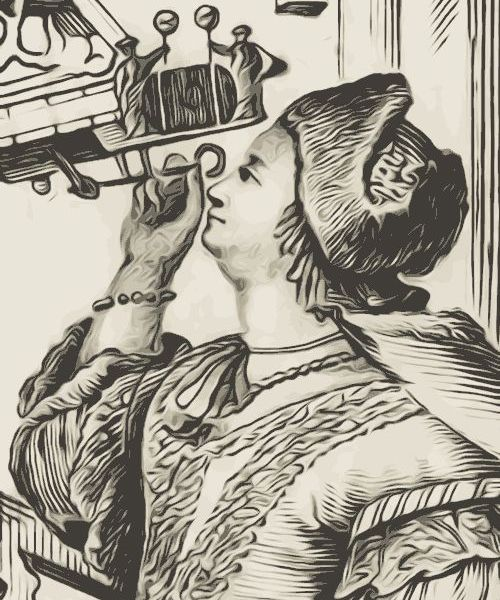
\includegraphics[width=10cm]{img/2026/elisabetha_hevelius.jpg}};
			%
			\draw [fill=galaxy, ultra thick] (4.6,-5.1) rectangle (11.4,-6.2);
			\node at (8,-5.6) {\textcolor{black}{\fontsize{18}{19}\selectfont Elisabeth Hevelius}};
			%
			\draw [fill=title, thick] (14,6.85) rectangle (27,7.75);
			\node (example-textwidth-2) [right, align=left, text width=12cm, color=black, font=\fontsize{18pt}{19pt}\selectfont] at (15,7.35) {\textbf{17 gennaio 1647}};
			%
			\node (example-textwidth-2) [right, align=left, text width=11cm, color=black, font=\fontsize{18pt}{19pt}\selectfont] at (15,5.5) {Astronoma};
			%
			\draw [fill=dida, thick] (14,4.2) rectangle (27,-8.5);
			\node (example-textwidth-2) [right, align=left, text width=11cm, color=black, font=\fontsize{18pt}{19pt}\selectfont] at (15,-2.3) {\textbf{Elisabeth Koopmann} e' considerata la prima donna astronoma della storia.\\
			Figlia di una ricca famiglia di mercanti di Danzica, all'eta' di 16 anni sposo' il gia' all'epoca famoso astronomo \textbf{Johannes Hevelius}, che era al suo secondo matrimonio. La coppia ebbe quattro figli: un maschio, che mori' subito dopo la nascita, e tre femmine, che sopravvissero. Studio' il latino, in cui eccelleva, cosa che permise alla coppia di mantenere dei proficui rapporti con la comunita' scientifica, e in particolare astronomica dell'epoca.};
			%
			\node (example-textwidth-2) [right, align=left, text width=11cm, color=black, font=\fontsize{18pt}{19pt}\selectfont] at (15,-20) {Nelle illustrazioni dell'epoca (1673), si vede Elisabeth Hevelius osservare il cielo al sestante insieme con il marito, mostrando come i suoi coevi erano a conoscenza del suo ruolo nella ricerca astronomica. I due adottarono strumenti particolarmente avanzati per l'epoca, rendendo il loro osservatorio a Danzica uno dei piu' importanti d'Europa.\\
			I loro risultati vennero raccolti da Elisabeth dopo la morte del marito nel \emph{Prodromus Astronomiae}, un ricco catalogo con 1564 stelle. Oltre a rappresentare un significativo progresso nell'osservazione celeste, il trattato fece progredire la conoscenza astronomica durante il XVII secolo. Il suo ruolo andava ben oltre la semplice assistenza nella raccolta dati: collaboro' attivamente all'estensione dei complessi calcoli matematici e nello sviluppo delle metodologie relative alla stesura del catalogo stellare. I suoi contributi furono quantitativi e qualitativi, a dimostrazione di un approccio meticoloso e sistematico alla ricerca astronomica.};
			%
			\draw [fill=title, thick] (14,-31.6) rectangle (27,-32.6);
			\node (example-textwidth-2) [right, align=left, text width=12cm, color=black, font=\fontsize{18pt}{19pt}\selectfont] at (15,-32.1) {\textbf{22 dicembre 1693}};
		\end{scope}
		%
		% Mary Fairfax
		%
		\begin{scope}[shift={(0,-66.9)}]
			\foreach \i in {0,1,...,11}
			{
				\draw [fill=white, thick] (14.75+\i,8.8) rectangle (15.25+\i,9.3);
			}
			%
			\draw [thick] (3,6.5) rectangle (13,-5.5);
			\node at (8,0.5) {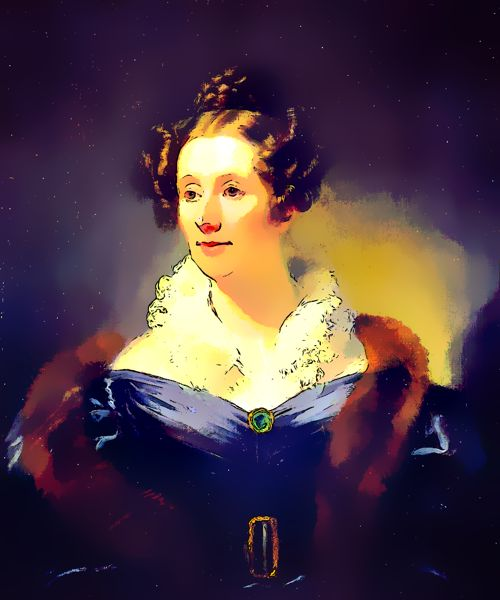
\includegraphics[width=10cm]{img/2026/mary_fairfax.jpg}};
			%
			\draw [fill=galaxy, ultra thick] (5.3,-5.1) rectangle (10.7,-6.1);
			\node at (8,-5.6) {\textcolor{black}{\fontsize{18}{19}\selectfont Mary Fairfax}};
			%
			\draw [fill=title, thick] (14,6.55) rectangle (27,7.45);
			\node (example-textwidth-2) [right, align=left, text width=12cm, color=black, font=\fontsize{18pt}{19pt}\selectfont] at (15,6.95) {\textbf{26 dicembre 1780}};
			%
			\node (example-textwidth-2) [right, align=left, text width=10cm, color=black, font=\fontsize{18pt}{19pt}\selectfont] at (15,5.6) {Matematica e astronoma};
			%
			\draw [fill=dida, thick] (14,4.5) rectangle (27,-6.1);
			\node (example-textwidth-2) [right, align=left, text width=10cm, color=black, font=\fontsize{18pt}{19pt}\selectfont] at (15,-0.8) {Si appassiono' alla scienza, in particolare alla matematica, sin dalla piu' tenera eta'. A ispirarla fu lo zio \textbf{Thomas Somerville}, che le raccontava le storie dei grandi scienziati dell'antichita'. Grazie al tutore del fratello minore, riusci' a ottenere una copia degli \emph{Elementi} di \textbf{Euclide}. Questa passione, pero', non era ben vista in famiglia, ma questo non scoraggio' Mary dal proseguire nei suoi interessi matematici.};
			%
			\node (example-textwidth-2) [right, align=left, text width=11cm, color=black, font=\fontsize{18pt}{19pt}\selectfont] at (15,-7) {Nel 1840 si sposo' con \textbf{Samuel Grieg}, che pero':};			
			%
			\shade [bottom color=paper02,top color=paper01] (14,-8.1) rectangle (27,-11.9);
			\draw [thick] (14,-8.1) rectangle (27,-11.9);
			\node (example-textwidth-2) [right, align=left, text width=11cm, color=black, font=\fontsize{18pt}{19pt}\selectfont] at (15,-10) {(...) aveva un’opinione molto bassa sulla capacita' del mio sesso, e non aveva alcuna conoscenza ne' interesse per le scienze di qualsiasi tipo.};
			%
			\node (example-textwidth-2) [right, align=left, text width=11cm, color=black, font=\fontsize{18pt}{19pt}\selectfont] at (15,-18) {Nel 1807 rimase vedova e, insieme con i suoi due figli, torno' in Scozia, dove prosegui' i suoi studi matematici, interessandosi in particolare alla trigonometria sferica e alle sezioni coniche. Studio' anche \emph{Astronomia} di \textbf{James Ferguson} e i \emph{Principia} di \textbf{Isaac Newton}. Nel 1811 ottenne la medaglia d'argento per la risoluzione di un'equazione diofantea proposta dalla rivista matematica del \emph{Military College} di Marlow. Inoltre pubblico' alcune soluziuoni sempre a equazioni diofantee nel \emph{Mathematical Repository}.};
			%
			\draw [fill=dida, thick] (14,-24) rectangle (27,-32);
			\node (example-textwidth-2) [right, align=left, text width=10cm, color=black, font=\fontsize{18pt}{19pt}\selectfont] at (15,-28) {Nel 1812 sposo' il cugino \textbf{William Somerville}, che la incoraggio' nel proseguire la sua attivita' scientifica. Grazie al marito venne a contatto con gli scienziati londinesi e, in particolare, coltivo' una lunga e proficua amicizia con \textbf{Ada Lovelace}, di cui divenne anche "maestra" e consigliera matematica.};
			%
			\node (example-textwidth-2) [right, align=left, text width=11cm, color=black, font=\fontsize{18pt}{19pt}\selectfont] at (15,-41) {Il suo primo articolo e' del 1826, \emph{On the magnetizing power of the more refrangible solar rays}, pubblicato sui \emph{Proceedings of the Royal Society}. A tal proposito c'era all'epoca la prassi di leggere gli articoli nel corso di un'assemblea della \emph{Royal Society}, ma non essendo questa aperta alle donne, fu il marito a leggerla per lei.\\
			Sarebbe troppo lungo citare tutti i suoi contributi, sia di ricerca, dove non rinunciava a sperimentare, sia nel campo della divulgazione scientifica. Tutta questa attivita', pero', le permise di diventare, nel 1835, membro onorario della \emph{Royal Astronomical Society} insieme con \textbf{Caroline Herschel}, prime donne a ottenere tale riconoscimento.\\
			La sua importanza fu tale che, dopo la sua morte, avvenuta a Napoli nel 1872, il \emph{Morning Post} scrisse:};
			%
			\shade [bottom color=paper02,top color=paper01] (14,-50.1) rectangle (27,-54.9);
			\draw [thick] (14,-50.1) rectangle (27,-54.9);
			\node (example-textwidth-2) [right, align=left, text width=11cm, color=black, font=\fontsize{18pt}{19pt}\selectfont] at (15,-52.5) {Per quante difficolta' potessimo incontrare a meta' del diciannovesimo secolo nello scegliere un re della scienza, non avevamo alcun dubbio sulla regina della scienza.};
			%
			\draw [fill=title, thick] (14,-55.4) rectangle (27,-56.3);
			\node (example-textwidth-2) [right, align=left, text width=12cm, color=black, font=\fontsize{18pt}{19pt}\selectfont] at (15,-55.9) {\textbf{29 novembre 1872}};
		\end{scope}
		%
		% Hertha Marks
		%
		\begin{scope}[shift={(0,-130.5)}]
			\foreach \i in {0,1,...,11}
			{
				\draw [fill=white, thick] (14.75+\i,6.4) rectangle (15.25+\i,5.9);
			}
			%
			\draw [thick] (3,4) rectangle (13,-8);
			\node at (8,-2) {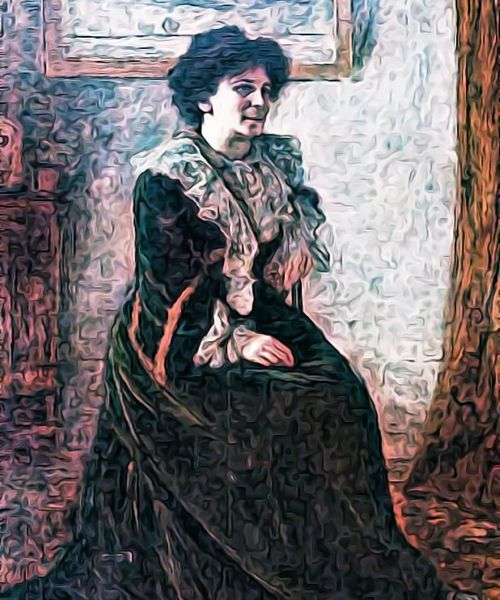
\includegraphics[width=10cm]{img/2026/hertha_ayrton.jpg}};
			%
			\draw [fill=galaxy, ultra thick] (5.3,-7.6) rectangle (10.7,-8.6);
			\node at (8,-8.1) {\textcolor{black}{\fontsize{18}{19}\selectfont Hertha Marks}};
			%
			\draw [fill=title, thick] (14,3.95) rectangle (27,4.85);
			\node (example-textwidth-2) [right, align=left, text width=12cm, color=black, font=\fontsize{18pt}{19pt}\selectfont] at (15,4.35) {\textbf{28 aprile 1854}};
			%
			\node (example-textwidth-2) [right, align=left, text width=10cm, color=black, font=\fontsize{18pt}{19pt}\selectfont] at (15,3) {Matematica, fisica, ingegnera};
			%
			\draw [fill=dida,thick] (14,2.2) rectangle (27,-7);
			\node (example-textwidth-2) [right, align=left, text width=11cm, color=black, font=\fontsize{18pt}{19pt}\selectfont] at (14.8,-2.4) {Nata \textbf{Phoebe Sarah Marks} da un orologiaio ebreo polacco e da una sarta, decise di adottare sin dall'adolescenza il nome di Hertha in onore dell'omonima eroina di una poesia di \textbf{Algernon Charles Swinburne} che criticava la religione organizzata.\\
			Studio' matematica con il fisico \textbf{Richard Glazebrook} e successivamente, grazie alla scrittrice \textbf{George Eliot}, riusci' a iscriversi al \emph{Girton College} a Cambridge.};
			%
			\node (example-textwidth-2) [right, align=left, text width=11cm, color=black, font=\fontsize{18pt}{19pt}\selectfont] at (15,-10.8) {Tra le tante attivita' che intraprese in quegli anni, costrui' anche uno sfigmomanometro, lo strumento utilizzato dai medici per misurare la pressione sanguigna. Poiche' in quegli anni Cambridge non rilasciava documenti accademici alle donne, si laureo' nel 1881 in matematica presso l'Universita' di Londra.};
			%
			\draw [fill=dida,thick] (14,-14.5) rectangle (27,-23.3);
			\node (example-textwidth-2) [right, align=left, text width=11cm, color=black, font=\fontsize{18pt}{19pt}\selectfont] at (14.8,-18.8) {Nella capitale inizio' a insegnare matematica e a ricamare per guadagnarsi da vivere, senza dimenticare pero' altre attivita' piu' interessanti, come la proposizione e risoluzione di problemi matematici e, soprattutto, l'invenzione di strumenti per cui richiese diversi brevetti (in totale furono 26). Il primo fu per un \emph{divisore di linea} (un calibro), datato 1884.};
			%
			\node (example-textwidth-2) [right, align=left, text width=11cm, color=black, font=\fontsize{18pt}{19pt}\selectfont] at (15,-26.8) {Nel 1891 inizio' una serie di ricerche sugli archi elettrici, che portarono alla pubblicazione di 12 articoli. Il lavoro portò a una dimostrazione pubblica avvenuta nel 1899 richiesta direttamente dalla \emph{Royal Society}. Venne cosi' descritta dal \emph{Daily News}:};
			%
			\shade [bottom color=paper02,top color=paper01] (14,-30.2) rectangle (27,-39.6);
			\draw [thick] (14,-30.2) rectangle (27,-39.6);
			\node (example-textwidth-2) [right, align=left, text width=11cm, color=black, font=\fontsize{18pt}{19pt}\selectfont] at (15,-34.8) {Cio' che stupi' le visitatrici... fu scoprire che una del loro sesso era responsabile dell'oggetto piu' pericoloso di tutti: una potente lampada ad arco racchiusa in un vetro. Mostro' con calma come, escludendo l'aria dalla lampada, se ne potesse prevenire il sibilo sgradevole e, proiettando sullo schermo un'immagine del carbone ardente, ne rese evidente la ragione anche ai piu' ottusi.};
			%
			%
			\node (example-textwidth-2) [right, align=left, text width=11cm, color=black, font=\fontsize{18pt}{19pt}\selectfont] at (15,-45.8) {Dopo un primo tentativo fallito nel 1902, divenne la prima donna a leggere un articolo scientifico presso la \emph{Royal Society}; nel 1904 lesse \emph{The Origin and Growth of Ripple Marks}. Nonostante questo fosse il primo di una serie di articoli, la \emph{Royal Society} non le concesse mai la \emph{fellowship}, pur assegnandole la \emph{Hughes Medal} nel 1906, prima donna a ottenere tale riconoscimento.\\
			Diede anche un contributo significativo nel corso della prima guerra mondiale inventando uno strumento non per uccidere, ma per salvare la vita ai soldati.};
			%
			\draw [fill=title, thick] (14,-52.1) rectangle (27,-53.1);
			\node (example-textwidth-2) [right, align=left, text width=12cm, color=black, font=\fontsize{18pt}{19pt}\selectfont] at (15,-52.6) {\textbf{26 agosto 1923}};
		\end{scope}
		% image credits
		\begin{scope}[shift={(0,-188)}]
			\draw [fill=space,thick] (2,1) rectangle (28,-1);
			%
			\node (example-textwidth-2) [right, align=left, text width=25cm, color=white, font=\fontsize{18pt}{19pt}\selectfont] at (2.5,0) {Le immagini sono tratte da Wikipedia e poi rielaborate graficamente usando il filtro G'MIC-Qt di Krita.};
		\end{scope}
		%
		\begin{scope}[shift={(0,-190)}]
			\node at (27,0) () {
\includegraphics[width=3.7cm]{licenza}};
			\node (example-textwidth-2) [right, align=left, text width=14cm, color=black, font=\fontsize{14pt}{15pt}\selectfont] at (12.5,-0.1) {Testo e grafica: @ulaulaman - Gianluigi Filippelli};
		\end{scope}
	\end{tikzpicture}
\end{document}
